\documentclass[10pt]{article}
\usepackage{soul}
\usepackage{fullpage,course}
\usepackage{hyperref}
\usepackage{enumerate}
\usepackage{xcolor}
\usepackage{listings}
\usepackage{graphicx} 
\usepackage{subcaption}
\usepackage{cleveref}
\usepackage{booktabs}
\usepackage[T1]{fontenc}

\lstset{
    basicstyle=\ttfamily\small,
    frame=single,
    numbers=left,
    numberstyle=\tiny,
    breaklines=true,
    columns=fullflexible
}

\def\handout{Machine Project II}
\parskip 6pt
\parindent 0pt

\begin{document}

\vspace*{-0.2in}

\begin{center}
\bf Student Name: \hl{Zirui Zhou} \hspace{3mm} NetID: \hl{ziruiz8}
\end{center}

\normalsize

\section{GPU}

\subsection{Part I}

\begin{enumerate}
	\item Suppose we use $A_{ij}$ to denot the element in matrix $A$. For reduction we have $$O_j=\sum_i A_{ij},$$ so the einsum notation could be $ij\to j$.
	\item For convolution we have $$O_{ij}=\sum_{k,l} A_{i+k,j+l}B_{kl},$$ so the einsum notation could be $ijkl,kl\to ij.$ Since standard einsum cannot express arithmetic on indices, there is no way to express the convolution operation in einsum notation.
	\item For batch matrix multiplication we have $$O_{ijl}=\sum_k A_{ijk}B_{ikl},$$ so the einsum notation could be $ijk,ikl\to ijl.$
	\item For \texttt{Relu} we have $$O_{ij}=\max(A_{ij},0),$$ so the einsum notation could be $ij\to ij.$ Since Einsum cannot apply arbitrary nonlinear functionsn such as $\max(x, 0)$, there is no way to express the \texttt{Relu} operation in einsum notation.
	\item For the elementwise multiplication we have $$O_{ijk}=A_{ijk}B_{ijk},$$ so the einsum notation could be $ijk,ijk\to ijk.$
\end{enumerate}

\subsection{Part II}

\begin{enumerate}
	\item The TCG of original computation is shown in \Cref{fig:mp2-1}.
	\item \label{item:r1-r2} After applying $R1$ then $R2$, the TCG is shown in \Cref{fig:mp2-2}.
	\item \label{item:r2-r1} After applying $R2$ then $R1$, the TCG is shown in \Cref{fig:mp2-3}. Note that $R1$ is not applicable after $R2$ here.
	\item The difference is that in \Cref{fig:mp2-3} there is still \texttt{O1}, while in \Cref{fig:mp2-2} \texttt{O1} is substituted by a new matrix multiplication. This is because in \Cref{fig:mp2-2} we first apply $R1$ that could substitute \texttt{O1} with a new matrix multiplication, while in \Cref{fig:mp2-3} we first apply $R2$ and it breaks the pattern that $R1$ could be applied to \texttt{O1}. 
	\item First do the shape analysis. We have $$A:[N,M], B:[M,K], C:[U,N], D:[N,V].$$ For \Cref{fig:mp2-2}, the addition and multiplication times is $\Theta(UN(M+V)+UMK)$. For \Cref{fig:mp2-3}, the addition and multiplication times is $\Theta(NMK+UN(K+V))$ If \Cref{fig:mp2-2} is better than \Cref{fig:mp2-3}, we have $$UM(N+K)<NK(U+M).$$ There are many possible values of $U, M, N, K$ that could satisfy this inequality. For example, when $U$ is extremely smaller than $M,N$ and $K$, we have $UM(N+K)\approx M(N+K)<NMK$ and $NK(U+M)\approx NMK$.
	
	Note that the profitability condition does not relate to $V$. This is because rule $R2$ does not reduce the computation strength, so the profitability condition is only related to the computation strength change by applying $R1$.
\end{enumerate}

\begin{figure}[ht]
    \centering

    \begin{subfigure}[b]{0.32\textwidth}
        \centering
        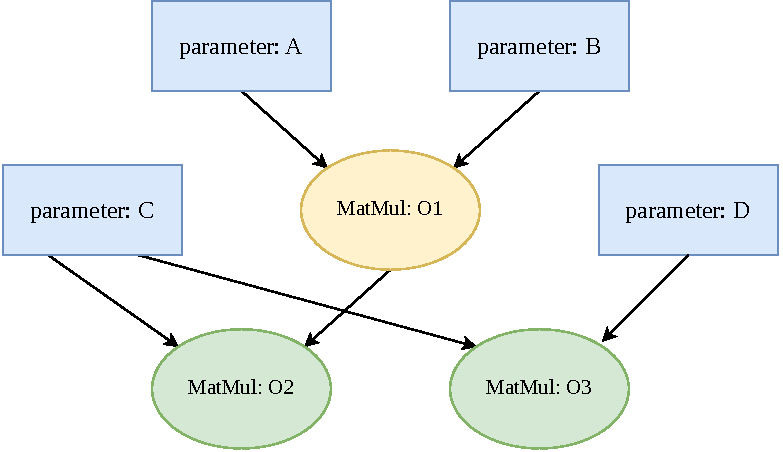
\includegraphics[width=\textwidth]{./fig/mp2-1.pdf}
        \caption{Original computation.}
        \label{fig:mp2-1}
    \end{subfigure}
    \hfill
    \begin{subfigure}[b]{0.32\textwidth}
        \centering
        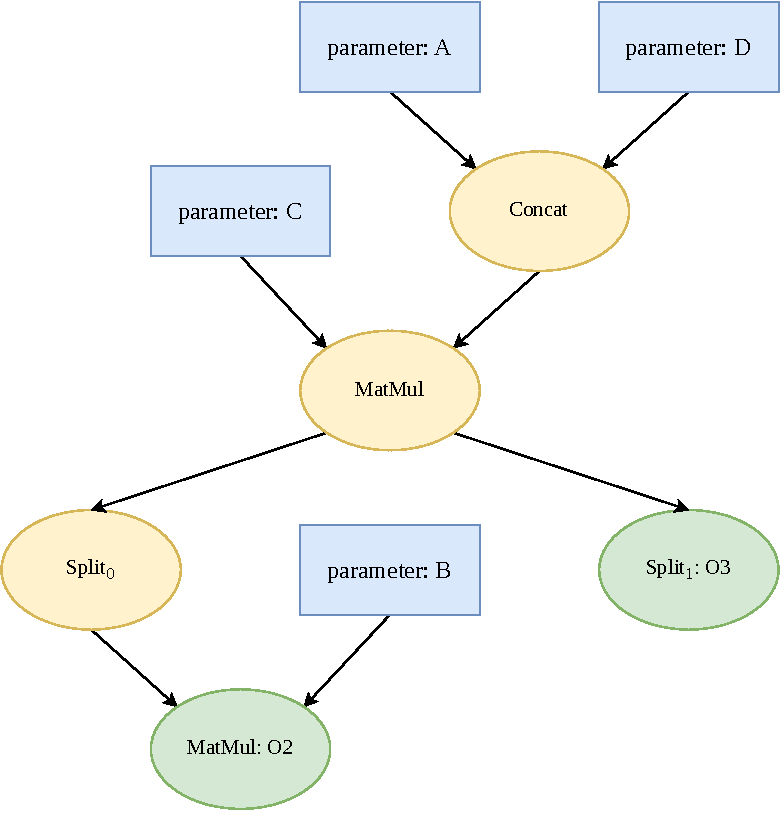
\includegraphics[width=\textwidth]{./fig/mp2-2.pdf}
        \caption{Applying first $R1$ then $R2$.}
        \label{fig:mp2-2}
    \end{subfigure}
    \hfill
    \begin{subfigure}[b]{0.32\textwidth}
        \centering
        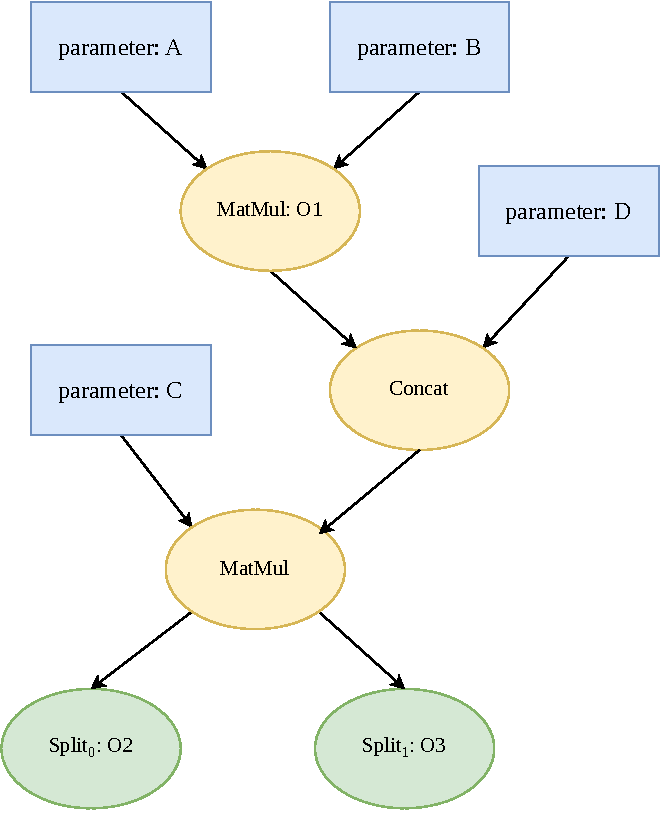
\includegraphics[width=\textwidth]{./fig/mp2-3.pdf}
        \caption{Applying first $R2$ then $R1$. Note that $R1$ is not applicable after $R2$ here.}
        \label{fig:mp2-3}
    \end{subfigure}

    \caption{TCG of Computation.}
    \label{fig:tcg}
\end{figure}

\subsection{Part III}

\end{document}
